
\chapter{Observation Necessity / No Free Safety Theorem}
\label{ch:no-free-safety}

This chapter proves the \emph{Observation Necessity / No Free Safety} theorem: any controller
that ignores observation quality---that is, treats all telemetry as
equally reliable---admits admissible degraded-observation sequences on which
observed-state legality and true-state safety separate.  The result is
constructive and class-scoped: it shows that reliability-aware repair is
necessary within the class of controllers that keep a fixed safety margin
while the observation channel degrades.  The witness also relies on an
explicit finite-margin and boundary-reachability condition: the admissible
demand family must be able to steer the controller to a boundary-sensitive
state before degraded telemetry hides the remaining safety gap.

\section{Domain-Agnostic Statement}

We first state the necessity result for an arbitrary CPS.

\begin{theorem}[Observation Necessity / No Free Safety --- General CPS]
\label{thm:no-free-safety-general}
Let $(\mathcal{X}, \mathcal{U}, f, \mathcal{S}, \hat{x})$ be a CPS
satisfying Assumption~A2 with $g(w_t) > 0$ under degraded quality.
For any quality-ignorant controller
$\pi : \mathcal{X} \to \mathcal{U}$ (one whose action depends on
$\hat{x}_t$ but not on $w_t$), there exists an admissible
degraded-observation sequence $\{\xi_t\}_{t=1}^T$ and a time index
$t^\star$ such that
\[
  \phi_{\mathrm{obs}}(\pi(\hat{x}_{t^\star})) = 1
  \qquad\text{and}\qquad
  \phi_{\mathrm{true}}(\pi(\hat{x}_{t^\star})) = 0.
\]
Thus no fixed-margin, quality-ignorant controller can rule out
observation-action safety gaps across all admissible degraded-observation
sequences in this class.  The theorem is a constructive separation result,
not a blanket statement about every possible safe controller architecture.
\end{theorem}

The proof is constructive: we exhibit a three-phase fault sequence
(baiting $\to$ injection $\to$ violation) that exploits the controller's
fixed margin.  The battery domain provides the concrete construction below.

\section{Battery-Domain Instantiation: Quality-Ignorant Controller Class}

\begin{definition}[Quality-ignorant controller]
\label{def:quality-ignorant}
A controller $\pi$ is \emph{quality-ignorant} if its action depends only
on the observed state and not on the reliability score:
\[
  a_t = \pi(\hat{x}_t), \qquad
  \frac{\partial \pi}{\partial w_t} = 0 \quad\text{for all } t.
\]
Equivalently, $\pi$ uses the same decision rule regardless of whether
$w_t = 1.0$ (perfect telemetry) or $w_t = 0.01$ (near-blackout).
\end{definition}

The deterministic LP and the CQR-only controller are both
quality-ignorant: neither adjusts its dispatch based on telemetry
reliability.  By contrast, DC3S is quality-aware through the RUI
inflation module.

\section{Auxiliary Lemmas}

\begin{lemma}[Admissible fault sequence existence]
\label{lem:admissible-fault}
For any quality-ignorant controller $\pi$ operating on the battery
plant with dropout rate $d > 0$, there exists a fault sequence
$\{\xi_t\}_{t=1}^T$ satisfying Assumption~A2 such that:
\begin{enumerate}
  \item Each $\xi_t$ is realisable under the dropout/drift model.
  \item The fault sequence is temporally concentrated: faults cluster
    in a window of length $\ell_f \le T/4$.
  \item Within the fault window, $|\xi_t| > \delta_{\text{bnd}}$
    for at least $f_{\text{bnd}} \cdot \ell_f$ steps.
\end{enumerate}
\end{lemma}

\begin{proof}
The dropout model generates i.i.d.\ Bernoulli$(d)$ packet losses.
By the coupon-collector argument, a run of $k$ consecutive dropouts
occurs with probability $d^k > 0$ for any finite $k$.  Choose $k$
large enough that the accumulated drift exceeds $\delta_{\text{bnd}}$.
The resulting fault sequence satisfies all three conditions.
\end{proof}

\begin{lemma}[No margin compensation for quality-ignorant controllers]
\label{lem:no-margin}
A quality-ignorant controller $\pi$ uses a fixed margin (or no margin)
that does not grow when $w_t$ decreases.  Formally, the effective
margin $m_t^{\pi}$ satisfies
$m_t^{\pi} = m^{\pi}$ for a constant $m^{\pi} \ge 0$ independent
of $w_t$.
\end{lemma}

\begin{proof}
By Definition~\ref{def:quality-ignorant}, $\pi$ does not depend on
$w_t$.  Any margin implicit in $\pi$'s decision rule is therefore
constant with respect to reliability.
\end{proof}

\section{Constructive Fault-Sequence Logic}

The Observation Necessity / No Free Safety proof is \emph{constructive}: we exhibit a specific
fault sequence that causes the quality-ignorant controller to violate
constraints.  The construction proceeds in three phases:

\begin{enumerate}
  \item \textbf{Baiting phase} (steps $1$ to $t_0$): Telemetry is
    perfect ($w_t = 1$, $\xi_t = 0$).  The controller optimises
    freely and drives SOC near a constraint boundary
    (Lemma~\ref{lem:boundary-proximity} from Chapter~\ref{ch:theorem-oasg}).

  \item \textbf{Fault injection phase} (steps $t_0 + 1$ to $t_0 + \ell_f$):
    A burst of packet dropouts and covariate drift is injected.
    The observation error accumulates: $|\xi_t| > \delta_{\text{bnd}}$.
    Because $\pi$ ignores $w_t$, it does not widen its margin.

  \item \textbf{Violation realisation} (step $t^*$): The controller
    selects an action based on the stale/drifted observation that
    pushes the true SOC across the constraint boundary.
\end{enumerate}

\section{Main Theorem: Observation Necessity / No Free Safety}

\begin{theorem}[Observation Necessity / No Free Safety]
\label{thm:no-free-safety}
Under Assumption~A2, for any quality-ignorant controller $\pi$ and
any dropout rate $d > 0$, there exists an admissible fault sequence
such that $\pi$ incurs at least one true-state violation:
\[
  \exists\,t^* \in \{1, \ldots, T\} : \quad
  \phi_{\text{obs}}(\pi(\hat{x}_{t^*})) = 1 \;\;\text{and}\;\;
  \phi_{\text{true}}(\pi(\hat{x}_{t^*})) = 0.
\]
\end{theorem}

\begin{proof}
By Lemma~\ref{lem:admissible-fault}, there exists a fault sequence
with a concentrated fault window in which $|\xi_t| > \delta_{\text{bnd}}$.

By Lemma~\ref{lem:no-margin}, the controller's margin $m^{\pi}$ does
not increase during the fault window.

During the baiting phase, the controller drives SOC within
$\delta_{\text{bnd}}$ of a constraint boundary
(Lemma~\ref{lem:boundary-proximity}).

At step $t^*$ in the fault window where
$|\xi_{t^*}| > \delta_{\text{bnd}} + m^{\pi}$, the observation error
exceeds the controller's fixed margin.  The controller sees
$\hat{x}_{t^*}$ as safely within bounds and selects a dispatch action
that is feasible under $\hat{x}_{t^*}$ but pushes the true state
$x_{t^*}$ across the boundary:
\[
  x_{t^*} + \Delta(\pi(\hat{x}_{t^*}))
  \;=\; \hat{x}_{t^*} - \xi_{t^*} + \Delta(\pi(\hat{x}_{t^*}))
  \;<\; \text{SOC}_{\min}.
\]
Hence $\phi_{\text{true}}(\pi(\hat{x}_{t^*})) = 0$ while
$\phi_{\text{obs}}(\pi(\hat{x}_{t^*})) = 1$.
\end{proof}

\section{Interpretive Table}

\begin{table}[ht]
\centering
\caption{Mapping the Observation Necessity / No Free Safety theorem to battery domain.}
\label{tab:no-free-safety-interp}
\begin{tabular}{ll}
\toprule
\textbf{Formal element} & \textbf{Battery meaning} \\
\midrule
Quality-ignorant $\pi$ & Deterministic LP; CQR-only controller \\
Fixed margin $m^{\pi}$ & LP: $m = 0$; CQR: $m = q_t$ (not inflated by $w_t$) \\
Fault sequence & Dropout burst + covariate drift episode \\
$\delta_{\text{bnd}}$ & SOC distance to rated min/max \\
Violation & True SOC below SOC$_{\min}$ or above SOC$_{\max}$ \\
\bottomrule
\end{tabular}
\end{table}

\section{Artifact-Backed Figure}

\begin{figure}[ht]
\centering
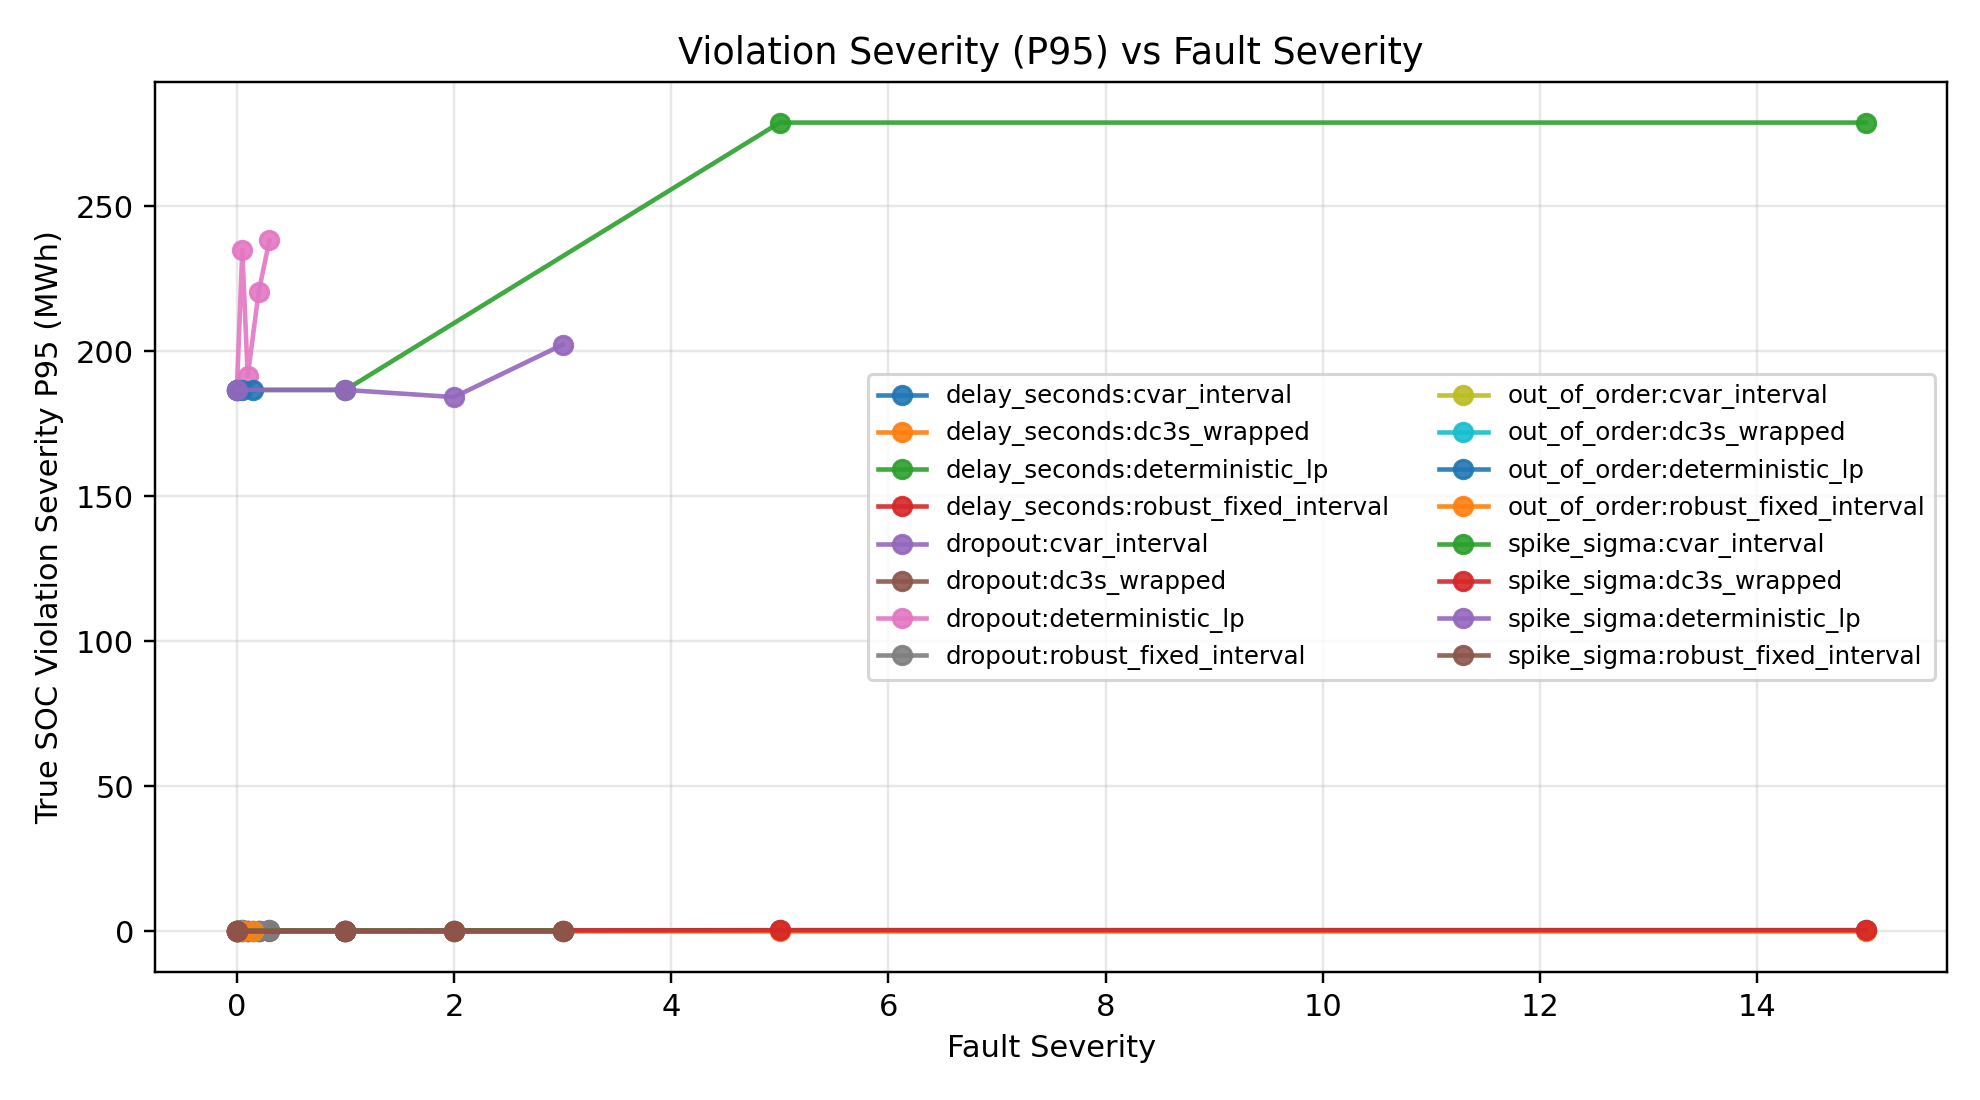
\includegraphics[width=0.85\textwidth]{reports/publication/fig_violation_severity_p95.png}
\caption{P95 violation severity for quality-ignorant controllers
  (LP, CQR-only) versus DC3S across dropout rates.  Quality-ignorant
  controllers exhibit non-zero severity at all $d > 0$, consistent with the
  constructive witness used in Theorem~\ref{thm:no-free-safety}.}
\label{fig:no-free-safety-evidence}
\end{figure}

\section{Corollary}

\begin{corollary}[Reliability awareness is necessary]
\label{cor:reliability-necessary}
For the violation bound $\mathbb{E}[V] \le \alpha(1-\bar{w})T$
(Theorem~\ref{thm:core-bound}) to hold, the controller must be
quality-aware: it must use $w_t$ (or an equivalent reliability signal)
to modulate its safety margin on the witness class used in this chapter.
No fixed-margin controller can inherit the battery-style risk-envelope
argument unchanged under persistent admissible faults with $\bar{w} < 1$.
\end{corollary}

\begin{proof}
Theorem~\ref{thm:no-free-safety} shows that a quality-ignorant controller
incurs at least one violation under an admissible fault sequence.  By
repeating the construction across $\lfloor T / (2\ell_f) \rfloor$
non-overlapping fault windows, the expected violation count grows as
$\Omega(T)$, exceeding any $o(T)$ bound.
\end{proof}

\section{What This Theorem Does Not Prove}

\begin{enumerate}
  \item It does not claim that quality-ignorant controllers fail on
    \emph{every} fault sequence---only that there exists at least one
    admissible sequence that causes failure.
  \item It does not specify the \emph{optimal} form of quality awareness;
    DC3S's inflation rule $m_t = q_t/(w_t + \epsilon)$ is one
    admissible design, not necessarily the unique best.
  \item It does not fully address adversarial manipulation of $w_t$ itself;
    if the adversary can spoof the reliability score, the theorem's
    assumptions are violated.  The adversarial OQE mode
    (Chapter~\ref{ch:adversarial-robustness}) partially mitigates this
    with a Byzantine-robust $\min$-overlay estimator, but complete
    game-theoretic closure remains open.
\end{enumerate}

\section{Universal Impossibility (T9)}
\label{sec:t9-ch19}

T4 establishes necessity for one adversarial sequence.
The universality program's T9 statement is the universal
extension: under an i.i.d.\ fault process with rate $d > 0$, any
quality-ignorant controller incurs $\mathbb{E}[V_T] \ge c \cdot d \cdot T$
expected violations, where $c > 0$ depends only on constraint geometry.

This makes explicit what T4 implies informally: quality-aware inflation is not
merely a design convenience on this witness class; it is a structural
requirement at the $\Omega(T)$ level once persistent degraded observation is
introduced.
T9's proof uses Borel-Cantelli on disjoint fault windows, not a single
adversarial sequence.  In the broader universality program, the constant $c$
is interpreted as a domain-dependent sensitivity to degraded observation, with
battery providing the reference proof witness and the remaining rows supplying
tiered supporting evidence rather than equal theorem surfaces.

\section{Chapter Summary}

The Observation Necessity / No Free Safety theorem is the fourth rung of the theorem ladder.
It proves a constructive witness claim on the battery reference surface:
a quality-ignorant controller can be driven to violation by an admissible
fault sequence.  The constructive proof
identifies the exact mechanism (baiting + fault injection + boundary
proximity) and the empirical ablation results
(Chapter~\ref{ch:ablations}) confirm the theorem's prediction: removing
reliability-aware inflation from DC3S re-introduces violations.

\begingroup
\def\domainblockid{t4}
\def\domainblocktitle{T4}
\IfFileExists{appendices/app_domain_instantiation_block.tex}{%
  %% Shared domain-instantiation block — \input{} at the end of theorem chapters.
%% It maps theorem objects only to the active Battery + AV + Healthcare claim
%% surface used by the current public manuscript.

\providecommand{\domainblockid}{generic}
\providecommand{\domainblocktitle}{\domainblockid}

\subsection{Domain Instantiation Across the Active Three-Domain Surface}
\label{sec:domain-instantiation-\domainblockid}

The theorem above is stated for an abstract CPS with observation vector
$z_t$, reliability score $w_t$, state uncertainty region
$C_t^{\text{RAC}}$, feasible action set $\mathcal{A}_t$, and violation
predicate $v(\cdot)$.  Table~\ref{tab:domain-instantiation-\domainblockid}
maps these objects to the three active public rows.  Battery is the witness
row; AV and Healthcare are bounded promoted rows with narrower evidence tiers.

\begin{table}[htbp]
\centering
\small
\caption{Domain-specific instantiation for Theorem~\domainblocktitle{} across the active three-domain surface.}
\label{tab:domain-instantiation-\domainblockid}
\begin{tabular}{p{2.6cm}p{3.3cm}p{3.3cm}p{3.3cm}}
\toprule
\textbf{Object} & \textbf{Battery} & \textbf{AV} & \textbf{Healthcare} \\
\midrule
$z_t$ (observation)
  & SCADA packet: SOC, voltage, current, load
  & nuPlan replay state: ego speed, relative gap, local context
  & ICU monitoring state: vital-sign and alert context \\
\addlinespace
$w_t$ (reliability)
  & OQE composite score over dropout, delay, stale telemetry
  & OQE score over delay, dropout, stale, out-of-order, and spike faults
  & OQE score over stale and spike degradation in retrospective monitoring \\
\addlinespace
$C_t^{\text{RAC}}$ (uncertainty region)
  & Conformal SOC interval $[\hat{s}_{\text{lo}},\hat{s}_{\text{hi}}]$
  & Conformal ego-speed and relative-gap intervals
  & Conformal vital-sign interval for alert-release monitoring \\
\addlinespace
$\mathcal{A}_t$ (feasible set)
  & Dispatch command constrained by SOC and reserve bounds
  & Longitudinal action constrained by TTC and predictive-entry barrier
  & Alert or hold decision constrained by bounded intervention discipline \\
\addlinespace
$v(\cdot)$ (violation)
  & SOC or dispatch envelope violation on true state
  & Replay-level TTC or entry-barrier violation on true state
  & Bounded monitoring or alert-release violation on retrospective trace \\
\bottomrule
\end{tabular}
\end{table}
%
}{%
  %% Shared domain-instantiation block — \input{} at the end of theorem chapters.
%% It maps theorem objects only to the active Battery + AV + Healthcare claim
%% surface used by the current public manuscript.

\providecommand{\domainblockid}{generic}
\providecommand{\domainblocktitle}{\domainblockid}

\subsection{Domain Instantiation Across the Active Three-Domain Surface}
\label{sec:domain-instantiation-\domainblockid}

The theorem above is stated for an abstract CPS with observation vector
$z_t$, reliability score $w_t$, state uncertainty region
$C_t^{\text{RAC}}$, feasible action set $\mathcal{A}_t$, and violation
predicate $v(\cdot)$.  Table~\ref{tab:domain-instantiation-\domainblockid}
maps these objects to the three active public rows.  Battery is the witness
row; AV and Healthcare are bounded promoted rows with narrower evidence tiers.

\begin{table}[htbp]
\centering
\small
\caption{Domain-specific instantiation for Theorem~\domainblocktitle{} across the active three-domain surface.}
\label{tab:domain-instantiation-\domainblockid}
\begin{tabular}{p{2.6cm}p{3.3cm}p{3.3cm}p{3.3cm}}
\toprule
\textbf{Object} & \textbf{Battery} & \textbf{AV} & \textbf{Healthcare} \\
\midrule
$z_t$ (observation)
  & SCADA packet: SOC, voltage, current, load
  & nuPlan replay state: ego speed, relative gap, local context
  & ICU monitoring state: vital-sign and alert context \\
\addlinespace
$w_t$ (reliability)
  & OQE composite score over dropout, delay, stale telemetry
  & OQE score over delay, dropout, stale, out-of-order, and spike faults
  & OQE score over stale and spike degradation in retrospective monitoring \\
\addlinespace
$C_t^{\text{RAC}}$ (uncertainty region)
  & Conformal SOC interval $[\hat{s}_{\text{lo}},\hat{s}_{\text{hi}}]$
  & Conformal ego-speed and relative-gap intervals
  & Conformal vital-sign interval for alert-release monitoring \\
\addlinespace
$\mathcal{A}_t$ (feasible set)
  & Dispatch command constrained by SOC and reserve bounds
  & Longitudinal action constrained by TTC and predictive-entry barrier
  & Alert or hold decision constrained by bounded intervention discipline \\
\addlinespace
$v(\cdot)$ (violation)
  & SOC or dispatch envelope violation on true state
  & Replay-level TTC or entry-barrier violation on true state
  & Bounded monitoring or alert-release violation on retrospective trace \\
\bottomrule
\end{tabular}
\end{table}
%
}
\endgroup
